% Matlab编程基础

% 未完成:编程语言的种类等可以参考 cplusplus 网站
\textbf{Matlab(Matrix Laboratory)}的中文名叫矩阵实验室,是一款著名的科学计算软件,也指这个软件中使用的编程语言.这里仅介绍最基本的 Matlab 功能和语法,且仅介绍本书使用到的功能.如果只需要了解本书的算法而不想使用 Matlab,可略过界面相关的介绍.

% 此处应有版权,然而中国的学生版停止发售了..都不知道怎么写了.

\subsection{界面介绍}

\begin{figure}[ht]
\centering
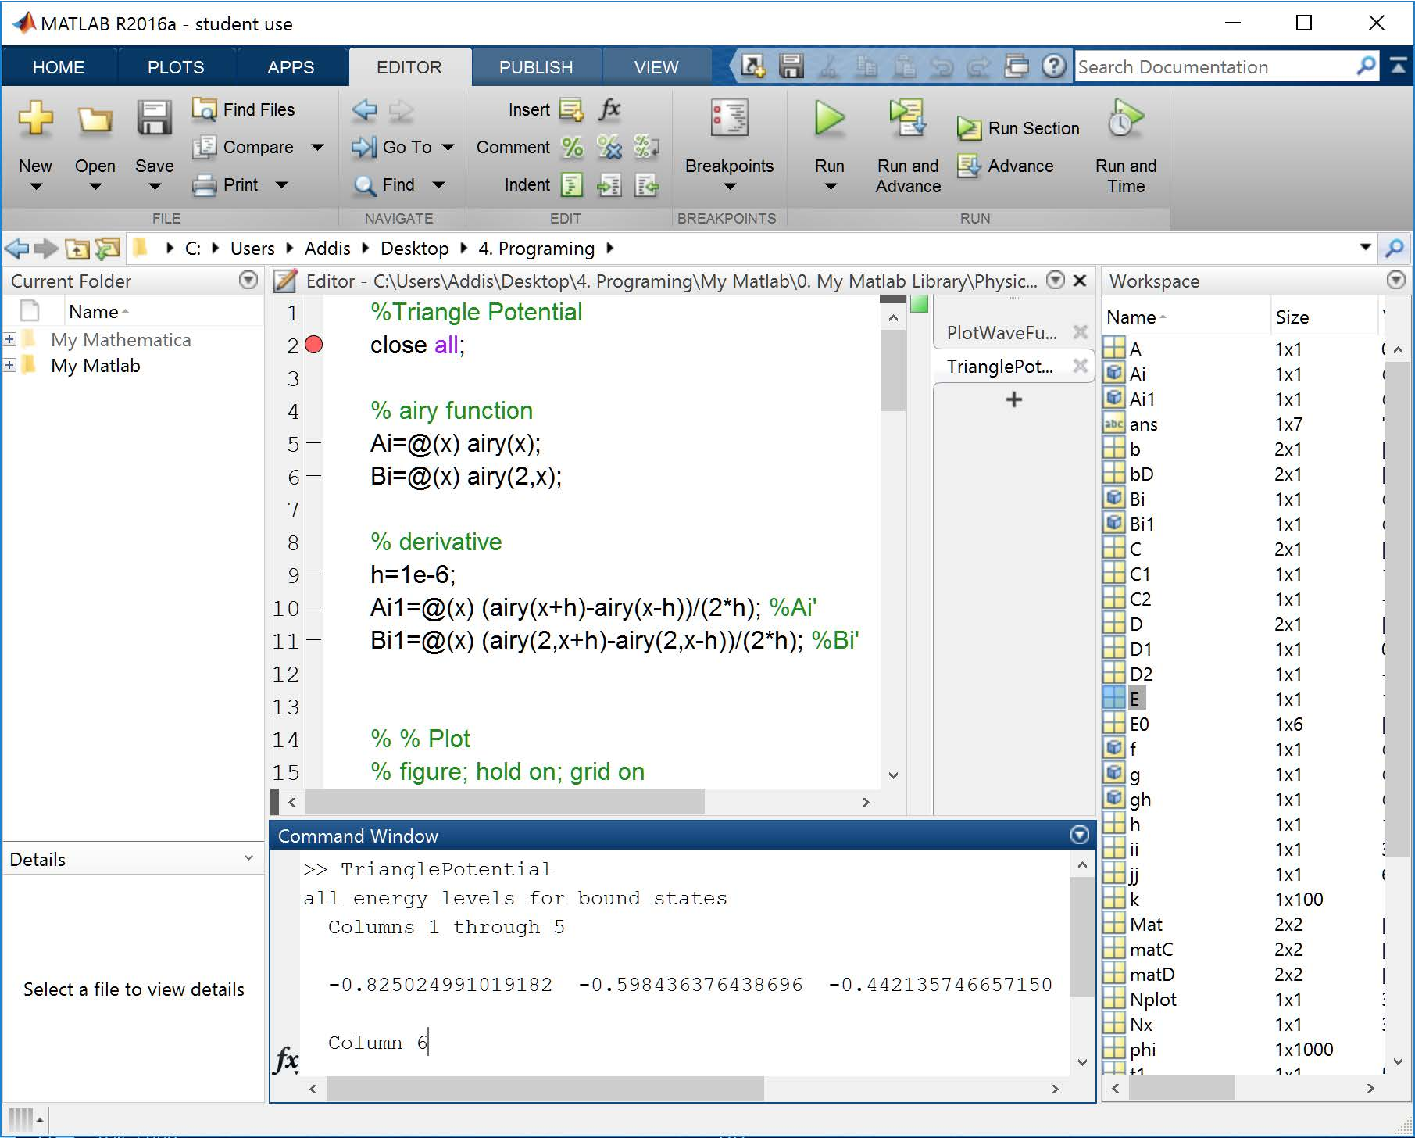
\includegraphics[width= 14cm]{./figures/Matlab1.pdf}
\caption{Matlab 的 IDE 界面}\label{Matlab_fig1}
\end{figure}

Matlab 的编程界面(\autoref{Matlab_fig1})属于\textbf{集成开发环境(IDE/Integrated Develop Environment)},简而言之就是一切与 Matlab 编程有关的工作都可以在该界面完成\footnote{界面语言默认与操作系统语言相同,本书使用英文界面.}.以下介绍界面中常用的窗口.要选择显示的窗口,可在 Home 菜单中点击 Layout 按钮,并在 Show 下面勾选需要的窗口.

\textbf{Editor} 用于编辑代码,同时具有自动检测语法错误,代码调试等功能.Matlab 的代码文件分为脚本文件和函数文件两种形式,后缀名都为 m,用图1中 Editor 菜单栏的 Save 按钮可保存代码文件.Matlab 作为一种\textbf{解释语言(Interpreted Language)}可以直接在 Editor 中运行源代码,无需传统的编译过程.为了让 Matlab 能运行代码文件,需要把文件所在的目录\footnote{在英文界面下 Matlab 不能识别中文目录,建议用英文命名文件夹.}添加到 Matlab 的搜索路径下.

\begin{figure}[ht]
\centering
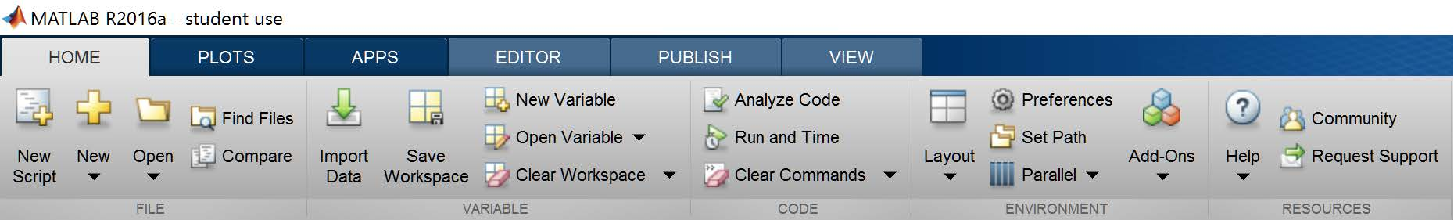
\includegraphics[width= 14cm]{./figures/Matlab2.pdf}
\caption{Home 菜单}\label{Matlab_fig2}
\end{figure}

如\autoref{Matlab_fig2},Home 菜单中的 Set Path 按钮可以设置 Matlab 的搜索路径.点开后用 Add Folder 按钮可以添加单个文件夹(不包含子文件夹),用 Add with Subfolders 添加文件夹(包含子文件夹).用 Remove 删除已添加的路径,用 Default 还原初始设置,用 Save 保存修改,用 Close 关闭窗口.若要运行程序,回到 Editor 菜单点击 Run 按钮即可.

\textbf{Command Window} 主要用于输入临时指令或者调试程序,可输入除了函数定义外的任意指令.Command Window 只能按输入顺序执行,不方便修改和编辑,如果指令较长或有多个指令,应该使用 Editor.在 Command Window 中按回车执行输入的指令,按上箭头可重复已输入的指令.

\textbf{Workspace} 用于查看 Matlab 当前的所有变量的列表.Matlab 的所有变量都可以理解为矩阵,单个值可理解为 $1\times 1$ 的矩阵.列表中 Name 是变量名,Size 是矩阵维度,Value 是变量值,右上角的下拉菜单中的 Choose Columns 中还可设置显示更多属性,例如 Bytes 是占用字节数,Class 是变量类型,Min 是最小值,Max 是最大值,Mean 是平均值,Median 是中位数,Std 是标准差等.双击 Workspace 中的变量可显示变量值.

% 还是应该先介绍语法再介绍文件形式!
\subsection{计算器}
下面我们仅用 Command Window 来熟悉 Matlab 的基本语法.我们先看如何把 Matlab 当做普通的科学计算器使用.
\begin{Command}
>> 1.2/3.4 + (5.6+7.8)*9 -1 \\
ans = 119.9529 \\
>> 1/exp(1) \\
ans = 0.3679 \\
>> exp(-1i*pi)+1 \\
ans = 0
\end{Command}
常用的运算符号有
\begin{Command}
+,-,*,/,\^\ (指数)
\end{Command}
常用的数学函数有
\begin{Command}
sqrt(开方),exp,sin,cos,tan,cot,asin,acos,atan,acot,real(实部),imag(虚部),conj(共轭)
\end{Command}
等(三角函数前面加 a 代表其反函数).运算的优先顺序与数学上的习惯一样.注意这些函数的自变量都可以是复数.为了区分虚数单位 \texttt{i} 和变量 \texttt{i},好习惯是在 \texttt{i} 前面加数字(上面的第三条命令).

\texttt{mod(N,n)} 是求余运算,计算 \texttt{N} 被 \texttt{n} 整除后的余数.注意这个函数有两个变量,用逗号隔开.要注意在 Matlab 中,这种有输入和输出的命令都是广义的\textbf{函数(function)},不仅是数学函数.

用大写 \texttt{E} 或小写 \texttt{e} 表示科学计数法(不允许有空格),如 $2.997\times 10^8$ 表示为 \texttt{2.997e8} 或 \texttt{2.997e+8}.用小写 \texttt{pi} 表示圆周率,用 \texttt{exp(1)} 表示自然对数底,用 \texttt{1+2i} 或 \texttt{1+2j} 等表示复数,注意 \texttt{i} 和 \texttt{j} 前面不能有空格.

如果需要多位小数,可使用 \texttt{format long} 命令使结果显示为\textbf{双精度}(约16位有效数字),用 \texttt{format short} 命令恢复默认格式.
\begin{Command}
>> format long; pi \\
ans = 3.141592653589793 \\
>> exp(1) \\
ans = 2.718281828459046
\end{Command}

\subsection{变量与矩阵}
\textbf{变量(variable)}可用于传递数据.变量名可以用含有多个字母,数字和下划线,注意变量名区分大小写,且首字符只能是字母.用等号对变量赋值,变量必须在等号左边,等号右边的运算结果会储存在变量中,直到再次被赋值.
\begin{Command}
>> a = 1.2/3.4 + (5.6+7.8)*9 -1 \\
a = 119.9529 \\
>> b = atan(a + 1) \\
b = 1.5625
\end{Command}
如果新的变量第一次被赋值,它会自动出现在 Workspace 窗口中.注意 Workspace 中的一个特殊的变量 \texttt{ans},如果命令的输出结果没有赋值给变量,就会自动赋值给 \texttt{ans}.注意一般不要对 \texttt{ans} 赋值.

另外,如果在命令后面加分号(semicolon)“\,;”,则命令执行后不输出结果.也可以用分号把多个命令写到一行.在以后用 Editor 编写程序时,每个命令后面都需要加分号,用 diplay 函数在 Command Window 显示结果.
\begin{Command}
>> 1 + 1; a = ans\^{}2 \\
a = 4
\end{Command}
用 \texttt{clear} 命令清空 Workspace 中的所有变量,用 \texttt{clear <var1>,<var2> ...} 清除指定的变量(\texttt{<var1>,<var2>}是变量名).用 \texttt{clc} 清空 Command Window (上箭头仍然可以查看历史命令).

本书只涉及到 3 种\textbf{变量类型(class)}:\textbf{双精度(double)},\textbf{字符(char)} 和 \textbf{逻辑(logical).}

双精度变量用于储存数值,有效数字约为 16 位(如果是复数,实部和虚部各 16 位),取值范围约为 $10^{-308}$ 到 $10^{308}$. 如无变量类型声明,所有命令中出现的常数及储存数值的变量都为 double.

Matlab 中的所有变量都可以理解为\textbf{矩阵},单值变量(标量,scalar)可以理解为 $1\times 1$ 的矩阵,只有一行或一列的矩阵叫做\textbf{行矩阵(row vector)}和\textbf{列矩阵(column vector)}.一些简单的矩阵操作如下
\begin{Command}
>> a = [1,2,3] \\
a = 1\ \ 2\ \ 3
\end{Command}
用方括号创建矩阵,用逗号分隔每行的矩阵元,行矢量中逗号可省略
\begin{Command}
>> a = [1 2 3] \\
a = 1\ \ 2\ \ 3
\end{Command}
用分号分隔行
\begin{Command}
>> b = [1;2;3] \\
b = \par
1 \par
2 \par
3 \\
>> c = [1 2 3; 2 3 4; 3 4 5]\\
c = \par
1\ \ 2\ \ 3 \par
2\ \ 3\ \ 4 \par
3\ \ 4\ \ 5
\end{Command}
方括号还可以用来合并矩阵(注意矩阵尺寸必须合适)
\begin{Command}
>> d = [a;a] \\
d = \par
1\ \ 2\ \ 3 \par
1\ \ 2\ \ 3 \\
>> e = [a a] \\
e = \par
1\ \ 2\ \ 3\ \ 1\ \ 2\ \ 3
\end{Command}
用 \texttt{size} 函数获取矩阵尺寸,用 \texttt{numel} 函数获取矩阵元个数
\begin{Command}
>> size(d) \\
ans = 2\ \ 3 \\
>> size(d,1) \\
ans = 2 \\
>> numel(d) \\
ans = 6
\end{Command}
用 \texttt{zeros} 函数生成全零矩阵
\begin{Command}
>> zeros(2,3) \\
ans = \par
0\ \ 0\ \ 0 \par
0\ \ 0\ \ 0
\end{Command}
用 zeros([2,3]) 和 zeros(size(d)) 结果也相同.用 \texttt{ones} 可以生成全 1 矩阵,也可以乘以任意常数
\begin{Command}
>> ones(2,3)*5 \\
ans = \par
5\ \ 5\ \ 5 \par
5\ \ 5\ \ 5
\end{Command}
用 \texttt{eye(N)} 生成 $N\times N$ 的单位矩阵,用 \texttt{rand(M,N)} 生成随机矩阵,矩阵元从 0 到 1 均匀分布.用 \texttt{M:step:N} 生成等差数列(行矢量),例如
\begin{Command}
>> 1:2:10 \\
ans = 1\ \ 3\ \ 5\ \ 7\ \ 9 \\
>> 0:pi/3:pi*2 \\
ans = 0\ \ 1.0472\ \ 2.0944\ \ 3.1416\ \ 4.1888\ \ 5.2360\ \ 6.2832 \\
>> 10:-2:1 \\
ans = 10\ \ 8\ \ 6\ \ 4\ \ 2
\end{Command}
用 \texttt{linspace(x1,x2,Nx)} 生成指定首项尾项和项数的等差数列(行矢量)
\begin{Command}
>> linspace(0,pi,4) \\
ans = 0\ \ 1.0472\ \ 1.2566\ \ 2.0944\ \ 3.1416
\end{Command}
下面介绍矩阵运算.同规格的尺寸可以进行 \texttt{+} 和 \texttt{-} 运算,矩阵和标量也可以;矩阵乘法\texttt{*} 既可以把常数与矩阵相乘,也可以进行数学上的矩阵乘法;矩阵的幂“\texttt{\^{}}”相当于矩阵与自己多次相乘;“\texttt{/}”可以把矩阵除以一个常数.
\begin{Command}
>> a = [1 2; 3 4]; b = [1 -1; 2 -2]; \\
>> a + b \\
ans = \par
2\ \ 1 \par
5\ \ 2\\
>> a * b \\
ans = \par
5\ \ -5 \par
11\ \ -11
\end{Command}
若要两个尺寸相同,可进行\textbf{逐个元素运算},如
\begin{Command}
>> a .* b \\
ans = \par
1\ \ -2 \par
6\ \ -8\\
>> a.\^{}2 \\
ans = \par
1\ \ 4 \par
9\ \ 16 \\
>> a ./ b \\
ans = \par
1.0000\ \ -2.0000 \par
1.5000\ \ -2.0000
\end{Command}
单引号“\texttt{'}”可以使实数矩阵转置,或使复矩阵取厄米共轭.若需要对复矩阵转置,用“\texttt{.'}”即可.
\begin{Command}
>> c = a + 1i*b \\
c = \par
1.0000 + 1.0000i\ \ 2.0000 - 1.0000i \par
3.0000 + 2.0000i\ \ 4.0000 - 2.0000i \\
>> c' \\
ans = \par
1.0000 - 1.0000i\ \ 3.0000 - 2.0000i \par
2.0000 + 1.0000i\ \ 4.0000 + 2.0000i \\
>> c.' \\
ans = \par
1.0000 + 1.0000i\ \ 3.0000 + 2.0000i \par
2.0000 - 1.0000i\ \ 4.0000 - 2.0000i
\end{Command}
Matlab 自带的数学函数一般支持矩阵自变量,结果是该函数对每个矩阵元分别运算
\begin{Command}
>> cos(0:pi/4:pi)\\
ans = \par
1.0000\ \ 0.7071\ \ 0.0000\ \ -0.7071\ \ -1.0000
\end{Command}
用矢量运算可以使代码简短易懂,且提高计算效率.

字符型变量一般用于控制行输出结果或对生成的图片进行标注.把 \texttt{N} 个字符放在一对单引号内,可生成 \texttt{1 $\times$ N} 的字符类型数组.
\begin{Command}
>> str1 = '\!这是一个字符串'; str2 = 'this is a string' \\
>> [str1, ',', str2] \\
ans = \par
这是一个字符串, this is a string \\
>> numel(str) \\
ans = 24
\end{Command}
把双精度变类型变为字符串用 \texttt{num2str} 函数(注意“2”的读音与“to”相同,“num”代表“number”,“str”代表字符串“string”),通常用于与其他字符矩阵合并,如
\begin{Command}
>> number = 3; str = ['The number is ', num2str(number), '.'] \\
str = \par
The number is 3.
\end{Command}
若要在字符串中加入英文单引号,可用两个英文单引号表示.

逻辑变量只能具有 \texttt{0} 或 \texttt{1} 两个值,分别代表\textbf{假(false)}和\textbf{真(true)}.最常用的地方是判断语句 \texttt{if} 的后面以及获取矩阵元.逻辑算符有
\begin{Command}
>,>=(大于等于),<,<=,==(等于)
\end{Command}
可用于比较双精度数组,返回逻辑型数组
\begin{Command}
>> L = 1 + 1 > 3 \\
L = 0
\end{Command}
逻辑“与”,“或”,“非”算符分别为(仅用于逻辑标量)\texttt{\&\&,||,\texttilde}.例如
\begin{Command}
>> 1 > 0 \&\& 2 > 1 \\
ans = 1 \\
>> 1 > 0 || 2 < 1 \\
ans = 1
>> ~ (1 > 0)
\end{Command}
只有两边都为真时,与运算才能为真.至少有一边为真,或运算就为真.非运算把真假互换,注意必须要加括号.

\textbf{矩阵索引} 用于表示矩阵部分矩阵元,例如
\begin{Command}
>> a = [1 2 3; 4 5 6; 7 8 9]; \\
ans = \par
1\ \ 2\ \ 3 \par
4\ \ 5\ \ 6 \par
7\ \ 8\ \ 9 \\
>> a(1,2) \\
ans = 2 \\
>> a(2:3,1) \\
ans = \par
4 \par
7 \\
>> a(2:3,1:2) \\
ans = \par
4\ \ 5 \par
7\ \ 8 \\
>> a([2,3],[1,2]) \\
ans = \par
4\ \ 5 \par
7\ \ 8 \\
>> a(:,2) \\
ans = \par
2 \par
5 \par
8 \\
>> a(1:end-1,2:3) \\
ans = \par
2\ \ 3 \par
5\ \ 6
\end{Command}
其中 \texttt{end} 表示某维度的最大索引(仅在索引中有效).以上的格式可以归结为“在小括号中用逗号把行矢量隔开”.注意索引不仅可以用来取值,还可以放在等号左边赋值.
\begin{Command}
>> b = a; b(1:3) = a(2:4) \\
b = \par
4\ \ 2\ \ 3 \par
7\ \ 5\ \ 6 \par
2\ \ 8\ \ 9
\end{Command}
要求左边的矩阵元个数等于右边.唯一的例外是当右边为标量
\begin{Command}
b(1:3) = 0 \\
b = \par
0\ \ 2\ \ 3 \par
0\ \ 5\ \ 6 \par
0\ \ 8\ \ 9 
\end{Command}
我们还可以用单个索引
\begin{Command}
>> a(2:5)\\
ans = 4\ \ 7\ \ 2\ \ 5 \\
>> a(7:end)\\
ans = 3\ \ 6\ \ 9
\end{Command}
注意单个索引的顺序是先增加第一个维度(行标),再增加第二个维度(列标).

我们还可以用相同大小逻辑数组索引
\begin{Command}
>> mark = logical([1 0 0; 0 0 1; 1 0 0]); a(mark) \\
ans = \par 1 \par 7 \par 6
\end{Command}
逻辑索引常见的例子如
\begin{Command}
>> a(a-3 <= 1) \\
ans = \par 1 \par 4 \par 2 \par 3
\end{Command}
注意逻辑索引中不能使用双精度类型代替逻辑类型.

\subsection{脚本文件}
在讲解更复杂的程序结构前,我们先来看脚本文件.\textbf{脚本(script)文件} 是包含若干个指令的文件,文件后缀名为 m.脚本文件可以单独执行,也在其他文件或 Command Window 中被调用(记得设置搜索路径).后者相当于把被调用脚本的代码直接插入到调用指令处,调用指令就是脚本文件的文件名.脚本中的每条命令后面应该加分号以隐藏输出结果,若需要输出,用 \texttt{disp} 函数.该函数的自变量可以是字符串或矩阵.

在脚本文件中,可以在行首或命令后用百分号 \texttt{\%} 进行\textbf{注释(comment)}.注释是程序的说明,使程序更易读,在执行程序时会被忽略(\autoref{Matlab_fig1}).
\begin{Command}
>> disp('good'); a = 3; disp(['a = ',num2str(a)]) \\
good \\
a = 3
\end{Command}
注意即使使用了分号,\texttt{disp} 仍然会显示结果.

\subsection{判断结构}
现在来看一段代码(脚本文件)
\begin{lstlisting}[language=Matlab]
a = rand(1,1); b = 0.5;
if a > b
    disp('a is larger');
else
    disp('b is larger');
end
\end{lstlisting}
不难猜测出这里的 \texttt{if} 用于判断,如果条件满足,则只执行 \texttt{if} 和 \texttt{else} 之间的指令.如果条件不满足,则只执行 \texttt{else} 到 \texttt{end} 的指令.以上程序随机生成从 0 到 1 的数,如果随机数大则输出第一段文字,否则输出第二段文字.
% 未完成:事实上前面还需要逻辑变量!以及介绍各种比较算符!

\subsection{循环结构}
% 未完成:前面还要讲矩阵的预赋值!
用 \texttt{for} 表示循环
\begin{lstlisting}[language=Matlab]
for ii = 1:3
    disp(['ii^2 = ' num2str(ii^2)]);
end
\end{lstlisting}
运行结果为
\begin{Command}
ii\^{}2 = 1 \\
ii\^{}2 = 4 \\
ii\^{}2 = 9 
\end{Command}
容易看出这段代码被执行了 3 次,\textbf{循环变量} \texttt{ii} 按顺序取 1:3 中的一个矩阵元.注意选取 \texttt{ii} 作为变量名是为了与虚数单位区分,也可以选择其他变量名.再来看一个稍复杂的循环
% 未完成:1:100 把中间的步长 1 省略了!
\begin{lstlisting}[language=Matlab]
Nx = 5;
x = zeros(1,Nx); 
x(1) = 2;
for ii = 2:numel(x)
    x(ii) = x(ii-1)^2;
end
disp(['x = ' num2str(x)])
\end{lstlisting}
在循环开始前 \texttt{x(1)} 被赋值为 2,在循环中,第 \texttt{ii} 个矩阵元 依次被赋值为第 \texttt{ii-1} 个矩阵元的平方.运行结果为
\begin{Command}
x = 2\ \ 4\ \ 16\ \ 256\ \ 65536
\end{Command}
注意在循环前用 \texttt{zero} 对矩阵进行了\textbf{预赋值(preallocation)}.预赋值不是必须的,但如果不进行预赋值,每次循环矩阵的尺寸都要改变,会导致程序运行变慢.另外注意循环中不允许给循环变量赋值.
% 未完成,嵌套循环

\subsection{函数文件}

我们已经学了一些函数,现在来看如何自定义函数.自定义函数需要一个单独的\textbf{函数文件}.的第一个命令必须是 function,用于定义主函数.文件名必须与主函数同名.文件中其他函数都是子函数.主函数可以调用子函数,子函数可以调用同文件中的其他子函数,但不能调用主函数,主函数和子函数都可以调用 Matlab 的内部函数或搜索路径下其他函数文件中的主函数.若函数文件在搜索路径下,其他 m 文件或 Command Window 中可以直接调用它的主函数.注意函数文件中的子函数不能从文件外被调用.函数的 workspace 是独立的,即 <定义函数的指令> 在执行的过程中,不能获取除 <变量> 外的变量,除非定义了全局变量(见 global). % 未完成
% 未完成,链接到函数的具体说明
注意函数只能通过函数文件定义,不能在脚本或控制行中定义.

\subsection{函数句柄(function handle)}
\textbf{函数句柄} 是一种特殊的变量类型,可用于定义一个临时的函数,也可传递到其他函数中.首先,对于已经存在的函数(包括函数文件定义的),可直接在函数名前面加 \texttt{@} 生成函数句柄
\begin{Command}
>> f = @sin \\
>> f(pi/2) \\
ans = 1;
\end{Command}
若函数由若干个运算组合而成,或包含若干其他变量,要在 \texttt{@} 后面指定函数句柄的变量
\begin{Command}
>> A = 3; w = 5; phi = pi/2; \\
>> f = @(x) A*sin(w*x+phi) + (2*x./pi).\^{}2; \\
>> f([0,pi/2]) \\
ans = \par
3.0000\ \ 1.0000; \\
f = @(x,phi) A*sin(w*x+phi) + (2*x./pi).\^{}2; \\
>> f([0,pi/2],pi/2) \\
ans = \par
3.0000\ \ 1.0000;
\end{Command}
注意这里用了逐个元素算符,使函数支持矩阵输入.

\subsection{自定义函数(function)}
格式为

[<输出1>,<输出2>,...] = function <函数名>(<变量1>,<变量2>...)

<定义函数的指令>

end

其中 <函数名> 是字母,数字和下划线的组合,例如 MyFun\_123,第一个字符不能是数字或下划线.若函数无变量,则小括号可省略.若函数无输出,则等号及方括号可省略.

函数的调用格式为 %这个不该出现这里!应该先学会调用系统函数

[<输出1>,<输出2>,...] = <函数名>(<变量1>,<变量2>...)
% 未完成: 如何忽略输入变量和输出变量,如何判断变量输入的个数等.

\subsection{程序调试}
\begin{figure}[ht]
\centering
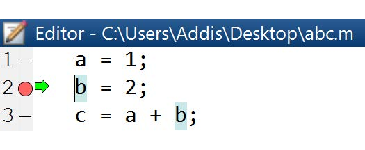
\includegraphics[width= 6cm]{./figures/Matlab3.pdf}
\caption{在行首设置 Breakpoint}\label{Matlab_fig3}
\end{figure}

若要调试程序,可选择一行代码并单击该行前面的横线,这时会出现红色圆点 Breakpoint (\autoref{Matlab_fig3}),程序运行到 Breakpoint 会暂停.

此时要查看变量情况,可通过 Workspace 查看各个变量的情况,也可用光标悬停在某个变量上.还可以用 Command Window 改变某些变量的值,或画图等.在这种调试状态下,也可以通过 Edit 菜单中的一些按钮控制接下来程序如何运行(\autoref{Matlab_fig4}).
\begin{figure}[ht]
\centering
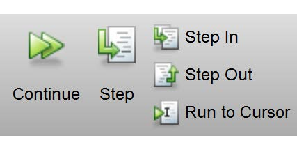
\includegraphics[width= 5cm]{./figures/Matlab4.pdf}
\caption{Step 菜单}\label{Matlab_fig4}
\end{figure}
其中“Continue”(快捷键 F5)是继续运行直到下一个 Breakpoint 或结束.“Step”(F10)是运行到下一行,“Step In”(F11)是进入子程序并暂停,“Step Out”是运行完当前子程序并回到子程序被调用的地方.“Run to Cursor”是运行到光标所在处.

\subsection{分节}
在行首用两个百分号“ \%\%” 可以对代码进行分节(\autoref{Matlab_fig5}).这样做一是可以使代码结构更清晰,二是可以单独选择某一节运行(Edit 菜单中的“Run Section”按钮).
\begin{figure}[ht]
\centering
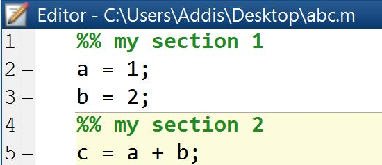
\includegraphics[width= 6cm]{./figures/Matlab5.pdf}
\caption{代码分节}\label{Matlab_fig5}
\end{figure}

\subsection{工具箱(Toolbox)}
在购买和安装 Matlab 软件时,可以选择各种各样的工具箱,常用的工具箱有曲线拟合(Curve Fitting,从离散的数据点得到一条曲线),图像处理(Image Processing,图像变换,增强,降噪,二值化等),图像获取(Image Acquisition,从相机获取图像),Matlab 编译器(MATLAB Compiler,编译代码,提高运行速度).注意使用了工具箱功能的代码在没有工具箱的 Matlab 软件上将无法运行.

\subsection{Matlab Online}
具有 Matlab 的基本功能,和类似于软件的界面,需要购买了正版 Matlab 的 Matlab 账号登录(学生账号也可以).若账号购买了工具箱(Toolbox),也可以使用对应的工具箱.本书官网提供免费的 Matlab 账号供读者试用和体验 Matlab Online,网址见本书封面或前言.



